\documentclass{beamer}
\usepackage{tikz,amsmath,hyperref,graphicx,stackrel,animate,amssymb,multirow}
\DeclareMathOperator{\tr}{tr}
\DeclareMathOperator*{\sg}{sg}
\usetikzlibrary{positioning,shadows,arrows,shapes,calc}
\newcommand{\argmax}{\operatornamewithlimits{argmax}}
\newcommand{\argmin}{\operatornamewithlimits{argmin}}
\newcommand{\average}{\operatornamewithlimits{average}}
\mode<presentation>{\usetheme{Frankfurt}}
\AtBeginSection[]
{
  \begin{frame}<beamer>
    \frametitle{Outline}
    \tableofcontents[currentsection,currentsubsection]
  \end{frame}
}
\title{Lecture 7: Matrix Calculus}
\author{Mark Hasegawa-Johnson\\These slides are in the public domain.}
\date{ECE 417: Multimedia Signal Processing, Fall 2023\\Much of this lecture is based on \url{https://en.wikipedia.org/wiki/Matrix_calculus}}  
\begin{document}

% Title
\begin{frame}
  \maketitle
\end{frame}

% Title
\begin{frame}
  \tableofcontents
\end{frame}

%%%%%%%%%%%%%%%%%%%%%%%%%%%%%%%%%%%%%%%%%%%%
\section{Notation}
\setcounter{subsection}{1}

\begin{frame}
  \frametitle{Notation}
  \begin{itemize}
  \item $x$ - a scalar
  \item $\mathbf{x}\in\Re^m$ - a column vector
  \item $\mathbf{x}^T\in\Re^n$ - a row vector
  \item $\mathbf{X}\in\Re^{m\times n}$ - a matrix
  \end{itemize}
\end{frame}

\begin{frame}
  \frametitle{Trace and Determinant}
  \begin{itemize}
  \item The trace of a matrix is the sum of its diagonal elements:
    \begin{displaymath}
      \tr(\mathbf{X})=\sum_i x_{i,i}
    \end{displaymath}
  \item The determinant of an $n\times n$ matrix is
    \begin{align*}
      \left|\mathbf{X}\right|
      &=\sum_{j=1}^n (-1)^{i+j} x_{i,j}\left|\mathbf{X}_{\neg i,\neg j}\right|~~\forall 1\le i\le n\\
      &=\sum_{i=1}^n (-1)^{i+j} x_{i,j}\left|\mathbf{X}_{\neg i,\neg j}\right|~~\forall 1\le j\le n
    \end{align*}
    where $\mathbf{X}_{\neg i,\neg j}$ is the submatrix computed by
    removing the $i^{\text{th}}$ row and $j^{\text{th}}$ column.  The
    determinant may also be written as the product of the eigenvalues:
    \begin{displaymath}
      \left|\mathbf{X}\right| = \sum_{i=1}^n \lambda_i(\mathbf{X})
    \end{displaymath}
  \end{itemize}
\end{frame}

\begin{frame}
  \frametitle{Norms of Vectors}
  \begin{itemize}
  \item The Lp norm of a vector is
    \begin{displaymath}
      \Vert\mathbf{x}\Vert_p=\left(x_1^p+x_2^p+\cdots+x_n^p\right)^{1/p}
    \end{displaymath}
  \item If the subscript is omitted, you may assume the L2 norm,
    a.k.a. the Euclidean norm:
    \begin{displaymath}
      \Vert\mathbf{x}\Vert
      =\Vert\mathbf{x}\Vert_2
      =\sqrt{x_1^2+x_2^2+\cdots+x_n^2}
    \end{displaymath}
  \item The Euclidean norm can also be calculated as the square root of the dot product
    of $\mathbf{x}$ with itself:
    \begin{displaymath}
      \Vert\mathbf{x}\Vert = \sqrt{\mathbf{x}^T\mathbf{x}}
    \end{displaymath}
  \end{itemize}
\end{frame}

\begin{frame}
  \frametitle{Norms of Matrices}
  \begin{itemize}
  \item The Frobenius norm of a matrix is the generalization of a Euclidean norm:
    \begin{displaymath}
      \Vert\mathbf{X}\Vert_F
      =\sqrt{\sum_i\sum_j |x_{i,j}|^2}
    \end{displaymath}
    It can be written in an interesting way:
    \begin{displaymath}
      \Vert\mathbf{X}\Vert_F=
      \sqrt{\tr(\mathbf{X}^T\mathbf{X})}
    \end{displaymath}
  \item The $L^p$ norm of a matrix is
    \begin{displaymath}
      \Vert\mathbf{X}\Vert_p=
      \sup_{\mathbf{v}}\frac{\Vert\mathbf{X}\mathbf{v}\Vert_p}{\Vert\mathbf{v}\Vert_p}
    \end{displaymath}
    These norms have cool mathematical properties, but they are not as
    useful in practice, usually, as the Frobenius norm.
  \end{itemize}
\end{frame}

%%%%%%%%%%%%%%%%%%%%%%%%%%%%%%%%%%%%%%%%%%%%
\section{Types of Derivatives}
\setcounter{subsection}{1}

\begin{frame}
  \frametitle{Types of derivatives}

  Let's talk about six types of derivatives:
  \centerline{\begin{tabular}{|c|c|ccc|}\hline
      \multicolumn{2}{|c|}{}&\multicolumn{3}{|c|}{Denominator}\\
      \multicolumn{2}{|c|}{}&Scalar & Vector & Matrix\\\hline
      \multirow{3}{*}{\rotatebox{90}{Numerator}} &
      Scalar &\rule{0pt}{15pt}
      $\frac{\partial y}{\partial x}$ &
      $\frac{\partial\mathbf{y}}{\partial x}$ &
      $\frac{\partial\mathbf{Y}}{\partial x}$ \\[5pt]
      &Vector &\rule{0pt}{15pt}
      $\frac{\partial y}{\partial\mathbf{x}}$ &
      $\frac{\partial\mathbf{y}}{\partial\mathbf{x}}$ &
      \\[5pt]
      &Matrix &\rule{0pt}{15pt}
      $\frac{\partial y}{\partial\mathbf{X}}$ &&\\[5pt]\hline
  \end{tabular}}
\end{frame}


%%%%%%%%%%%%%%%%%%%%%%%%%%%%%%%%%%%%%%%%%%%%
\section{Derivatives with Vectors}
\setcounter{subsection}{1}

\begin{frame}
  \frametitle{Vector-by-Scalar: the Tangent Vector}

  $\frac{\partial\mathbf{y}}{\partial x}$ is called the tangent vector:
  \begin{displaymath}
    \frac{\partial\mathbf{y}}{\partial x}=
    \left[\begin{array}{c}
        \frac{\partial y_1}{\partial x}\\
        \vdots\\
        \frac{\partial y_m}{\partial x}
      \end{array}\right]
  \end{displaymath}
\end{frame}

\begin{frame}
  \frametitle{Tangent Vector}
  \begin{columns}
    \begin{column}{0.5\textwidth}
      \begin{itemize}
      \item 
        Suppose that $x$ is scalar, and $\mathbf{y}=[y_1,y_2]^T$ is a
        point in a vector space.
      \item
        The function $\mathbf{y}(x)=[y_1(x),y_2(x)]^T$ sketches a
        curve in that space.
      \item
        The tangent vector is
        \begin{displaymath}
          \frac{\partial\mathbf{y}}{\partial x}=\left[\begin{array}{c}
              \frac{\partial y_1}{\partial x}\\
              \frac{\partial y_2}{\partial x}
            \end{array}\right]
        \end{displaymath}
      \end{itemize}
    \end{column}
    \begin{column}{0.5\textwidth}
      \centerline{\includegraphics[width=\textwidth]{exp/Tangent.png}}
      \url{https://commons.wikimedia.org/wiki/File:Tangent_to_a_curve.svg}
    \end{column}
  \end{columns}
\end{frame}

\begin{frame}
  \frametitle{Tangent Vector, Example \#1: Line}

  \centerline{\includegraphics[height=0.1\textheight]{exp/Ray.png}}
  
  Here is the equation for a line:
  \begin{displaymath}
    \mathbf{y}(x) = \mathbf{a}x = \left[\begin{array}{c}a_1x\\a_2x\end{array}\right]
  \end{displaymath}
  \ldots and here is its tangent vector:
  \begin{displaymath}
    \frac{\partial\mathbf{y}}{\partial x}
    = \mathbf{a}
  \end{displaymath}
\end{frame}
  
\begin{frame}
  \frametitle{Tangent Vector, Example \#2: Circle}
  \begin{columns}
    \begin{column}{0.5\textwidth}
      Here is the equation for a circle:
      \begin{displaymath}
        \mathbf{y}(\theta)=\left[\begin{array}{c}
          r\cos\theta\\r\sin\theta\end{array}\right]
      \end{displaymath}
      \ldots and here is its tangent vector:
      \begin{displaymath}
        \frac{\partial\mathbf{y}}{\partial\theta}=
        \left[\begin{array}{c}
            -r\sin\theta\\r\cos\theta
          \end{array}\right]
      \end{displaymath}
    \end{column}
    \begin{column}{0.5\textwidth}
      \centerline{\animategraphics[loop,controls,width=\textwidth]{20}{exp/circle_tangent-}{0}{100}}
      \url{https://commons.wikimedia.org/wiki/File:Circle\%2B3vectors_animated.gif}
    \end{column}
  \end{columns}
\end{frame}

\begin{frame}
  \frametitle{Rectifiable Curve}

  Suppose that $x$ is scalar, and $\mathbf{y}(x)=[y_1(x),y_2(x)]^T$ is
  a curve.  If $\frac{\partial\mathbf{y}}{\partial x}$ exists and is
  finite, then it is possible to calculate the length of the curve by
  integrating
  \begin{displaymath}
    \int \Vert\frac{\partial\mathbf{y}}{\partial x}\Vert dx
  \end{displaymath}
  \centerline{\animategraphics[loop,controls,height=0.3\textheight]{20}{exp/Arc_length-}{8}{28}}
  \url{https://upload.wikimedia.org/wikipedia/commons/d/dc/Arc_length.gif}
\end{frame}

\begin{frame}
  \frametitle{Tangent Vector, Example \#2: Circle}
  If $\mathbf{y}(\theta)=[r\cos\theta,r\sin\theta]^T$, its tangent is
  \begin{displaymath}
    \frac{\partial\mathbf{y}}{\partial\theta}=
    \left[\begin{array}{c}
        -r\sin\theta\\r\cos\theta
      \end{array}\right]
  \end{displaymath}
  The circumference of the circle is
  \begin{align*}
    c &= \int_{-\pi}^{\pi}\Vert\frac{\partial\mathbf{y}}{\partial\theta}\Vert d\theta\\
    &= \int_{-\pi}^{\pi}\sqrt{(-r\sin\theta)^2+(r\cos\theta)^2}d\theta\\
    &=\int_{-\pi}^\pi rd\theta= 2\pi r
  \end{align*}
\end{frame}

\begin{frame}
  \frametitle{Scalar-by-Vector: the Gradient}

  If $y$ is a scalar function of a vector $\mathbf{x}$, then $\nabla
  y$ is called the {\bf gradient}:
  \begin{align*}
    \nabla y &=
    \left[
      \begin{array}{c}
        \frac{\partial y}{\partial x_1}\\
        \vdots\\
        \frac{\partial y}{\partial x_m}
      \end{array}\right]
  \end{align*}
  Since $\frac{\partial\mathbf{y}}{\partial x}$ was a column vector,
  we will define $\frac{\partial y}{\partial\mathbf{x}}$ to be a row
  vector.  This is called ``numerator layout notation,'' and will have
  some benefits later on.
  \begin{align*}
    \frac{\partial y}{\partial\mathbf{x}}& =\nabla y^T
    =\left[\frac{\partial y}{\partial x_1},\ldots,\frac{\partial y}{\partial x_m}\right]\\
  \end{align*}
\end{frame}

\begin{frame}
  \frametitle{Directional Derivative}
  \begin{columns}
    \begin{column}{0.5\textwidth}
      Suppose $y(\mathbf{x})$ is a scalar function of a vector
      $\mathbf{x}=[x_1,x_2]^T$.  If $\mathbf{u}$ is any unit vector,
      then the {\bf directional derivative} of $y(\mathbf{x})$ in the
      $\mathbf{u}$ direction is written as
      \begin{align*}
        \nabla_{\mathbf{u}}y &=
        \nabla y^T \mathbf{u}\\
        &= \frac{\partial y}{\partial\mathbf{x}}\mathbf{u}\\
        &=
        \frac{\partial y}{\partial x_1}u_1+\frac{\partial y}{\partial x_2}u_2
      \end{align*}
    \end{column}
    \begin{column}{0.5\textwidth}
      \centerline{\includegraphics[width=\textwidth]{exp/Directional.png}}
      \url{https://commons.wikimedia.org/wiki/File:Directional_derivative_contour_plot.svg}
    \end{column}
  \end{columns}
\end{frame}

\begin{frame}
  \frametitle{Gradient Example \#1: Affine Function}
    \begin{columns}
    \begin{column}{0.5\textwidth}
      An affine function of $\mathbf{x}$ is written:
      \begin{align*}
        y(\mathbf{x}) &= \mathbf{a}^T\mathbf{x}+b\\
        &=a_1x_1+a_2x_2+b
      \end{align*}
      Its gradient is
      \begin{align*}
        \frac{\partial y}{\partial\mathbf{x}}
        &=\mathbf{a}^T
      \end{align*}        
    \end{column}
    \begin{column}{0.5\textwidth}
      \centerline{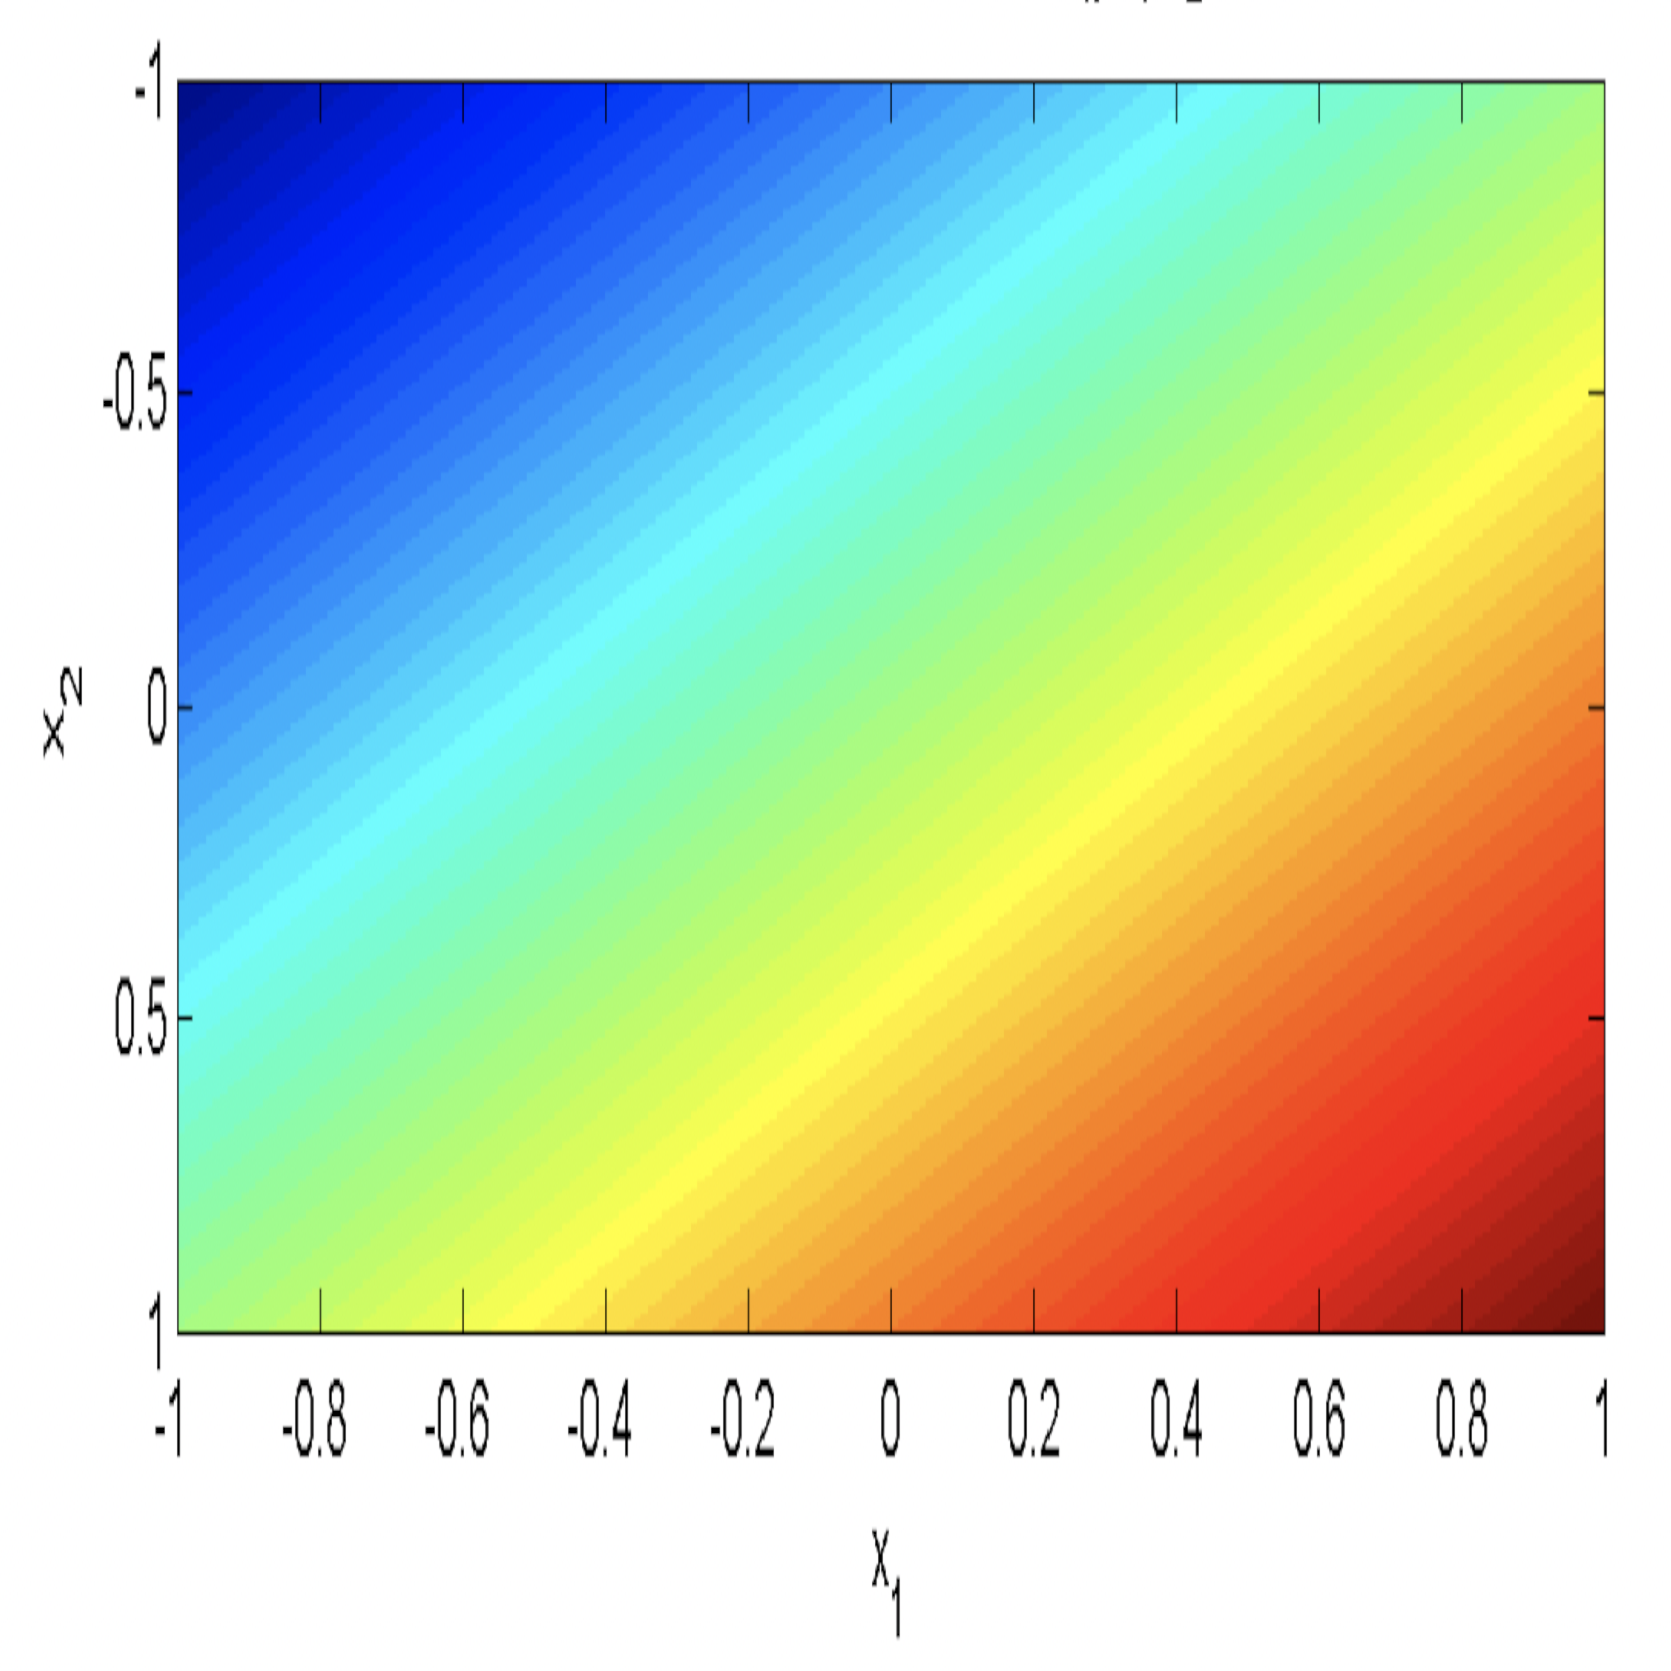
\includegraphics[width=\textwidth]{figs/constant_gradient.png}}
    \end{column}
  \end{columns}
\end{frame}


\begin{frame}
  \frametitle{Gradient Example \#2: Euclidean Norm}

  Consider the Euclidean norm of a vector:
  \begin{align*}
    \Vert\mathbf{x}\Vert^2=\mathbf{x}^T\mathbf{x}=x_1^2+\ldots+x_n^2
  \end{align*}
  By analogy to the affine function, setting
  $\mathbf{a}^T=\mathbf{x}^T$, we might think that
  $\frac{\partial\mathbf{x}^T\mathbf{x}}{\partial\mathbf{x}}=\mathbf{x}^T$. But
  from basic algebra, we know that
  \begin{align*}
    \frac{\partial(x_1^2+\ldots+x_n^2)}{\partial\mathbf{x}}
    &=\left[
      \frac{\partial(x_1^2+\ldots+x_n^2)}{\partial x_1},\ldots,
      \frac{\partial(x_1^2+\ldots+x_n^2)}{\partial x_n}
      \right]
    \\
    &=\left[2x_1,\ldots,2x_n\right]\\
    &=2\mathbf{x}^T
  \end{align*}
  What went wrong?
\end{frame}


\begin{frame}
  \frametitle{The Stop-Gradient Approach}

  One way to approach the problem of
  $\frac{\partial\mathbf{x}^T\mathbf{x}}{\partial\mathbf{x}}$ is the
  \textbf{stop-gradient} approach:
  \begin{enumerate}
  \item First, pretend that $\mathbf{x}^T$ is a constant vector that
    does not change when $\mathbf{x}$ changes --- in other words, stop
    the gradient w.r.t. $\mathbf{x}^T$.  We can write this as
    \begin{displaymath}
      \frac{\partial\sg(\mathbf{x}^T)\mathbf{x}}{\partial\mathbf{x}}=
      \mathbf{x}^T
    \end{displaymath}
  \item Second, take the derivative w.r.t. $\mathbf{x}^T$ while
    stopping the gradient w.r.t.  $\mathbf{x}$:
    \begin{displaymath}
      \frac{\partial\mathbf{x}^T\sg(\mathbf{x})}{\partial\mathbf{x}^T}=
      \mathbf{x}
    \end{displaymath}
  \item Finally, realize that when $\mathbf{x}$ changes,
    $\mathbf{x}^T$ also changes, so we need to include both parts of
    the derivative:
    \begin{displaymath}
      \frac{\partial\mathbf{x}^T\mathbf{x}}{\partial\mathbf{x}}=
      \frac{\partial\sg(\mathbf{x}^T)\mathbf{x}}{\partial\mathbf{x}}+
      \left(\frac{\partial\mathbf{x}^T\sg(\mathbf{x})}{\partial\mathbf{x}^T}\right)^T=
      2\mathbf{x}^T
    \end{displaymath}
  \end{enumerate}
\end{frame}

\begin{frame}
  \frametitle{Gradient Example \#3: Linear Regression}
  \begin{columns}
    \begin{column}{0.5\textwidth}
      Linear regression is the problem of approximating $y_i$ as a linear function of $\mathbf{x}_i$:
      \begin{displaymath}
        y_i\approx \mathbf{a}^T\mathbf{x}_i,~~~1\le i\le n
      \end{displaymath}
      The approximation is computed by minimizing the mean-squared error:
      \begin{align*}
        {\mathcal{L}}&=\sum_{i=1}^n \left(y_i-\mathbf{x}_i^T\mathbf{a}\right)^2\\
        &=\sum_{i=1}^n \left(y_i^2-y_i\mathbf{a}^T\mathbf{x}_i-y_i\mathbf{x}_i^T\mathbf{a}+
        \mathbf{a}^T\mathbf{x}_i\mathbf{x}_i^T\mathbf{a}\right)
      \end{align*}
    \end{column}
    \begin{column}{0.5\textwidth}
      \centerline{\includegraphics[width=\textwidth]{exp/linear_regression.png}}
      \url{https://commons.wikimedia.org/wiki/File:Linear_least_squares_example2.svg}
    \end{column}
  \end{columns}
\end{frame}

\begin{frame}
  \frametitle{Gradient Example \#3: Linear Regression}

  \begin{align*}
    {\mathcal{L}}
    &=\sum_{i=1}^n \left(y_i^2-y_i\mathbf{a}^T\mathbf{x}_i-y_i\mathbf{x}_i^T\mathbf{a}+
    \mathbf{a}^T\mathbf{x}_i\mathbf{x}_i^T\mathbf{a}\right)
  \end{align*}
  We can solve for $\mathbf{a}$ by finding the derivative,
  $\frac{\partial\mathcal{L}}{\partial\mathbf{a}}$, and setting it
  equal to zero:
  \begin{align*}
    \frac{\partial\mathcal{L}}{\partial\mathbf{a}}
    &=
    \frac{\partial\mathcal{L}(\mathbf{a},\sg(\mathbf{a}^T))}{\partial\mathbf{a}}+
    \left(\frac{\partial\mathcal{L}(\sg(\mathbf{a}),\mathbf{a}^T)}{\partial\mathbf{a}^T}\right)^T\\
    &=\sum_{i=1}^n -2y_i\mathbf{x}_i^T+ 2\mathbf{a}^T\mathbf{x}_i\mathbf{x}_i^T
    &= 0\\
    \mathbf{a}
    &=\left(\sum_{i=1}^n\mathbf{x}_i\mathbf{x}_i^T\right)^{-1}\left(\sum_{i=1}^n\mathbf{x}_iy_i\right)
  \end{align*}
\end{frame}

\begin{frame}
  \frametitle{Vector-by-Vector: the Jacobian}

  If $\mathbf{y}(\mathbf{x})\in\Re^m$ is a vector function of a vector
  $\mathbf{x}\in\Re^n$, then
  $\frac{\partial\mathbf{y}}{\partial\mathbf{x}}$ is called the
  Jacobian.
  \begin{displaymath}
    \frac{\partial\mathbf{y}}{\partial\mathbf{x}}=
    \left[\begin{array}{ccc}
        \frac{\partial y_1}{\partial x_1} & \cdots & \frac{\partial y_1}{\partial x_n}\\
        \vdots&\ddots&\vdots\\
        \frac{\partial y_m}{\partial x_1} & \cdots & \frac{\partial y_m}{\partial x_n}
      \end{array}\right]
  \end{displaymath}
        
\end{frame}

\begin{frame}
  \frametitle{Jacobian Example: Affine Transformation}

  An affine transformation of a vector $\mathbf{x}$ is written as:
  \begin{align*}
    \mathbf{y}(\mathbf{x}) &= \mathbf{A}\mathbf{x}+\mathbf{b}\\
    &= \left[\begin{array}{c}
        a_{1,1}x_1+a_{1,2}x_2+b_1\\a_{2,1}x_1+a_{2,2}x_2+b_2
      \end{array}\right]
  \end{align*}
  Its Jacobian is:
  \begin{displaymath}
    \frac{\partial\mathbf{y}}{\partial\mathbf{x}}=\mathbf{A}
  \end{displaymath}
\end{frame}

\begin{frame}
  \frametitle{Chain Rule}

  The Jacobian is most useful because we can use it in the chain rule.
  Suppose that $\mathbf{z}\in\Re^p$ is a function of
  $\mathbf{y}\in\Re^n$, and $\mathbf{y}$ is a function of
  $\mathbf{x}\in\Re^m$.  Then
  \begin{align*}
    &\frac{\partial\mathbf{z}}{\partial\mathbf{x}}=
    \frac{\partial\mathbf{z}}{\partial\mathbf{y}}
    \frac{\partial\mathbf{y}}{\partial\mathbf{x}}\\
    &=
    \left[\begin{array}{ccc}
        \frac{\partial z_1}{\partial y_1} & \cdots & \frac{\partial z_1}{\partial y_n}\\
        \vdots&\ddots&\vdots\\
        \frac{\partial z_p}{\partial y_1} & \cdots & \frac{\partial z_p}{\partial y_n}
      \end{array}\right]
    \left[\begin{array}{ccc}
        \frac{\partial y_1}{\partial x_1} & \cdots & \frac{\partial y_1}{\partial x_m}\\
        \vdots&\ddots&\vdots\\
        \frac{\partial y_n}{\partial x_1} & \cdots & \frac{\partial y_n}{\partial x_m}
      \end{array}\right]
    &=
    \left[\begin{array}{ccc}
        \frac{\partial z_1}{\partial x_1} & \cdots & \frac{\partial z_1}{\partial x_m}\\
        \vdots&\ddots&\vdots\\
        \frac{\partial z_p}{\partial x_1} & \cdots & \frac{\partial z_p}{\partial x_m}
      \end{array}\right]
  \end{align*}
        
\end{frame}

\begin{frame}
  \frametitle{Summary: Derivatives with Vectors}
  \begin{align*}
    \frac{\partial\mathbf{a}x}{\partial x} &= \mathbf{a}\\
    \frac{\partial\mathbf{a}^T\mathbf{x}}{\partial\mathbf{x}} &= \mathbf{a}^T\\
    \frac{\partial\mathbf{x}^T\mathbf{x}}{\partial\mathbf{x}} &= 2\mathbf{x}^T\\
    \frac{\partial(y_i-\mathbf{a}^T\mathbf{x}_i)^2}{\partial\mathbf{a}}
    &= 2(\mathbf{a}^T\mathbf{x}_i-y_i)\mathbf{x}_i^T\\
    \frac{\partial\mathbf{A}\mathbf{x}}{\mathbf{x}}&= \mathbf{A}
  \end{align*}    
\end{frame}


%%%%%%%%%%%%%%%%%%%%%%%%%%%%%%%%%%%%%%%%%%%%
\section{Derivatives with Matrices}
\setcounter{subsection}{1}

\begin{frame}
  \frametitle{Matrix-by-Scalar: the Tangent Matrix}

  If $\mathbf{Y}(x)\in\Re^{m\times n}$ is a matrix function of a scalar $x$,
  we can compute a tangent matrix,
  $\frac{\partial\mathbf{Y}}{\partial x}$:
  \begin{displaymath}
    \frac{\partial\mathbf{Y}}{\partial x} =
    \left[\begin{array}{ccc}
        \frac{\partial y_{1,1}}{\partial x}&\cdots&\frac{\partial y_{1,n}}{\partial x}\\
        \vdots&\ddots&\vdots\\
        \frac{\partial y_{m,1}}{\partial x}&\cdots&\frac{\partial y_{m,n}}{\partial x}
      \end{array}\right]
  \end{displaymath}
\end{frame}

\begin{frame}
  \frametitle{Tangent Matrix Example \#1: Linear Scaling}

  Suppose that
  \begin{align*}
    \mathbf{Y}(x) &= \mathbf{A}x\\
    &=\left[\begin{array}{ccc}
        a_{1,1}x&\cdots&a_{1,n}x\\
        \vdots&\ddots&\vdots\\
        a_{m,1}x&\cdots&a_{m,n}x
      \end{array}\right]
  \end{align*}
  Then its tangent matrix is
  \begin{align*}
    \frac{\partial\mathbf{Y}}{\partial x} =\mathbf{A}
  \end{align*}
\end{frame}

\begin{frame}
  \frametitle{Tangent Matrix Example \#2: Rotation Matrix}
  \begin{columns}
    \begin{column}{0.5\textwidth}
      The rotation matrix, $\mathbf{T}(\theta)$, is the matrix that
      takes any input vector and rotates it by $\theta$ radians:
      \begin{displaymath}
        \mathbf{T}(\theta)=
        \left[\begin{array}{cc}
            \cos\theta & -\sin\theta\\
            \sin\theta & \cos\theta
          \end{array}\right]
      \end{displaymath}
    \end{column}
    \begin{column}{0.5\textwidth}
      \centerline{\includegraphics[width=\textwidth]{exp/rotation_matrix.png}}
      \url{https://commons.wikimedia.org/wiki/File:Visual_Derivation_of_Equations_For_Rotation_In_2D.svg}
    \end{column}
  \end{columns}
\end{frame}

\begin{frame}
  \frametitle{Tangent Matrix Example \#2: Rotation Matrix}
  The rotation matrix and its tangent are:
  \begin{displaymath}
    \mathbf{T}(\theta)=
    \left[\begin{array}{cc}
        \cos\theta & -\sin\theta\\
        \sin\theta & \cos\theta
      \end{array}\right],~~~~~
    \frac{\partial\mathbf{T}}{\partial\theta}= 
    \left[\begin{array}{cc}
        -\sin\theta & -\cos\theta\\
        \cos\theta & -\sin\theta
      \end{array}\right]
  \end{displaymath}
  One thing we can do with this is, by simple linearity, for any
  vector $\mathbf{v}(\theta)=\mathbf{T}(\theta)\mathbf{u}$, for a
  fixed initial $\mathbf{u}$, we can show that
  \begin{displaymath}
    \frac{\partial\mathbf{v}}{\partial\theta} =
    \frac{\partial\mathbf{T}(\theta)\mathbf{u}}{\partial\theta} =
    \left(\frac{\partial\mathbf{T}}{\partial\theta}\right)\mathbf{u}
  \end{displaymath}
\end{frame}

\begin{frame}
  \frametitle{Scalar-by-Matrix: the Gradient Matrix}

  $\frac{\partial y}{\partial\mathbf{X}}$ has no universally accepted
  name, but in machine learning it is often called the gradient
  matrix, in analogy with the gradient vector.  In {\bf numerator
    layout} order, $\mathbf{X}$ and $\partial y/\partial\mathbf{X}$
  are defined as:
  \begin{displaymath}
    \mathbf{X}=
    \left[\begin{array}{ccc}
        x_{1,1}&\cdots&x_{1,n}\\
        \vdots&\ddots&\vdots\\
        x_{m,1}&\cdots&x_{m,n}
      \end{array}\right],~~~~~
    \frac{\partial y}{\partial\mathbf{X}}=
    \left[\begin{array}{ccc}
        \frac{\partial y}{\partial x_{1,1}}&\cdots&\frac{\partial y}{\partial x_{m,1}}\\
        \vdots&\ddots&\vdots\\
        \frac{\partial y}{\partial x_{1,n}}&\cdots&\frac{\partial y}{\partial x_{m,n}}
      \end{array}\right]
  \end{displaymath}
\end{frame}

\begin{frame}
  \frametitle{Gradient Matrix Example \#1: Trace of X}

  For example, suppose $y=\tr(\mathbf{X})$:
  \begin{displaymath}
    y(\mathbf{X}) = \tr(\mathbf{X})= x_{1,1}+x_{2,2}+\cdots
  \end{displaymath}
  The gradient of the trace of a matrix is:
  \begin{displaymath}
    \frac{\partial y}{\partial\mathbf{X}} =
    \left[\begin{array}{ccc}
        \frac{\partial y}{\partial x_{1,1}}&
        \frac{\partial y}{\partial x_{2,1}}&
        \cdots\\
        \frac{\partial y}{\partial x_{1,2}}&
        \frac{\partial y}{\partial x_{2,2}}&
        \cdots\\
        \vdots&\vdots&\ddots
      \end{array}\right]=
    \left[\begin{array}{ccc}
        1&0&\cdots\\
        0&1&\cdots\\
        \vdots&\vdots&\ddots
      \end{array}\right]
  \end{displaymath}
  In other words,
  \begin{displaymath}
    \frac{\partial\tr(\mathbf{X})}{\partial\mathbf{X}} =I
  \end{displaymath}
\end{frame}

\begin{frame}
  \frametitle{Gradient Matrix Example \#1: Trace of AX}

  Now suppose $y=\tr(\mathbf{A}\mathbf{X})$, where
  $\mathbf{A}\in\Re^{n\times m}$ and $\mathbf{X}\in\Re^{m\times n}$.
  The $(i,j)^{\text{th}}$ element of the matrix $\mathbf{C}=\mathbf{A}\mathbf{X}$
  is $c_{i,j}=\sum_{k=1}^ma_{i,k}x_{k,j}$.  The trace is the sum along the main
  diagonal, so
  \begin{displaymath}
    y(\mathbf{X}) = \tr(\mathbf{A}\mathbf{X})= \sum_{i=1}^nc_{i,i}=
    \sum_{i=1}^n\sum_{k=1}^m a_{i,k}x_{k,i}
  \end{displaymath}
  The gradient of the trace of a matrix is:
  \begin{displaymath}
    \frac{\partial y}{\partial\mathbf{X}}=
    \left[\begin{array}{ccc}
        \frac{\partial y}{\partial x_{1,1}}&\cdots&\frac{\partial y}{\partial x_{m,1}}\\
        \vdots&\ddots&\vdots\\
        \frac{\partial y}{\partial x_{1,n}}&\cdots&\frac{\partial y}{\partial x_{m,n}}
      \end{array}\right]
    =
    \left[\begin{array}{ccc}
        a_{1,1}&\cdots&a_{1,m}\\
        \vdots&\ddots&\vdots\\
        a_{n,1}&\cdots&a_{n,m}
      \end{array}\right]=\mathbf{A}
  \end{displaymath}
  In other words,
  \begin{displaymath}
    \frac{\partial\tr(\mathbf{A}\mathbf{X})}{\partial\mathbf{X}} =\mathbf{A}
  \end{displaymath}
\end{frame}

\begin{frame}
  \frametitle{Gradient Matrix Example \#2: Pre- and Post-Multiplication}

  Suppose we pre-multiply by some vector $\mathbf{u}$, and
  post-multiply by some other vector $\mathbf{v}$:
  \begin{displaymath}
    y(\mathbf{X})=\mathbf{u}^T\mathbf{X}\mathbf{v}=
    \sum_{i=1}^m\sum_{j=1}^n u_ix_{i,j}v_j
  \end{displaymath}
  Then the gradient is:
  \begin{displaymath}
    \frac{\partial y}{\partial\mathbf{X}}=
    \left[\begin{array}{ccc}
        \frac{\partial y}{\partial x_{1,1}}&\cdots&\frac{\partial y}{\partial x_{m,1}}\\
        \vdots&\ddots&\vdots\\
        \frac{\partial y}{\partial x_{1,n}}&\cdots&\frac{\partial y}{\partial x_{m,n}}
      \end{array}\right]
    =\left[\begin{array}{ccc}
        u_1v_1&\cdots&u_mv_1\\
        \vdots&\ddots&\vdots\\
        u_1v_n&\cdots&u_mv_n
      \end{array}\right]
    = \mathbf{v}\mathbf{u}^T
  \end{displaymath}
  So the gradient of $\mathbf{u}^T\mathbf{X}\mathbf{v}$ is
  $\mathbf{v}\mathbf{u}^T$?  Why does that make sense?
\end{frame}

\begin{frame}
  \frametitle{The Trace Equality} It's time to introduce one more
  fundamental fact about linear algebra, called \textbf{the trace
    equality}.  For any compatibly-sized matrices
  $\mathbf{A}\in\Re^{m\times n}$ and $\mathbf{B}\in\Re^{n\times m}$,
  \begin{displaymath}
    \tr(\mathbf{AB})=\tr(\mathbf{BA})
  \end{displaymath}
\end{frame}

\begin{frame}
  \frametitle{The Trace Equality}
  \begin{displaymath}
    \tr(\mathbf{AB})=\tr(\mathbf{BA})
  \end{displaymath}
  \textbf{Proof:}
  \begin{itemize}
  \item The $(i,j)^{\text{th}}$ element of the matrix
    $\mathbf{C}=\mathbf{A}\mathbf{B}$ is $c_{i,j}=\sum_{k=1}^na_{i,k}b_{k,j}$.
    The trace sums the main diagonal, so
    \begin{displaymath}
      \tr(\mathbf{A}\mathbf{B})=\sum_{i=1}^mc_{i,i}
      =\sum_{i=1}^m\sum_{k=1}^n a_{i,k}b_{k,i}
    \end{displaymath}
  \item The $(j,k)^{\text{th}}$ element of the matrix 
    $\mathbf{D}=\mathbf{A}\mathbf{B}$ is $d_{j,k}=\sum_{i=1}^mb_{j,i}a_{i,k}$.
    The trace sums the main diagonal, so
    \begin{displaymath}
      \tr(\mathbf{B}\mathbf{A})=\sum_{k=1}^md_{k,k}=\sum_{k=1}^n\sum_{i=1}^m b_{k,i}a_{i,k}
    \end{displaymath}
  \item Those two things are the same.
  \end{itemize}
\end{frame}

\begin{frame}
  \frametitle{Gradient Matrix Example \#2: Pre- and Post-Multiplication}
  \begin{itemize}
  \item $\mathbf{u}^T\mathbf{X}\mathbf{v}$ is a scalar, so it is its own trace:
    \begin{displaymath}
      y(\mathbf{X})=\mathbf{u}^T\mathbf{X}\mathbf{v}=
      \tr\left(\mathbf{u}^T\mathbf{X}\mathbf{v}\right)
    \end{displaymath}
  \item By the trace equality,
    \begin{displaymath}
      y(\mathbf{X})=\tr\left(\mathbf{u}^T\mathbf{X}\mathbf{v}\right)=
      \tr\left(\mathbf{v}\mathbf{u}^T\mathbf{X}\right)
    \end{displaymath}
  \item So the gradient is:
    \begin{displaymath}
      \frac{\partial y}{\partial\mathbf{X}}=
      \frac{\partial\tr\left(\mathbf{v}\mathbf{u}^T\mathbf{X}\right)}{\partial\mathbf{X}}
      =
      \mathbf{v}\mathbf{u}^T
    \end{displaymath}
  \end{itemize}
\end{frame}

\begin{frame}
  \frametitle{Gradient Matrix Example \#3: Frobenius Norm Squared}

  There are several possible extensions of Euclidean norms to
  matrices, of which the Frobenius norm is the most useful.  The
  Frobenius norm squared is just the sum of the squares of all
  elements of the matrix:
  \begin{displaymath}
    \Vert\mathbf{X}\Vert_F^2
    =\sum_{i=1}^m\sum_{j=1}^n x_{i,j}^2
  \end{displaymath}
  From the definition of a matrix gradient, it's pretty obvious that
    \begin{displaymath}
      \frac{\partial\Vert\mathbf{X}\Vert_F^2}{\partial\mathbf{X}}=
      =\left[\begin{array}{ccc}
          2x_{1,1}&\cdots&2x_{m,1}\\
          \vdots&\ddots&\vdots\\
          2x_{1,n}&\cdots&2x_{m,n}
      \end{array}\right]=2\mathbf{X}^T
    \end{displaymath}
\end{frame}

\begin{frame}
  \frametitle{Gradient Matrix Example \#3: Frobenius Norm Squared}
    If you remember, the trace of $\mathbf{A}\mathbf{X}$ is
  \begin{displaymath}
    \tr(\mathbf{A}\mathbf{X})= \sum_{i=1}^n\sum_{k=1}^m a_{i,k}x_{k,i}
  \end{displaymath}
  If we choose $\mathbf{A}=\mathbf{X}^T$, then $a_{i,k}=x_{k,i}$, and
  therefore
  \begin{displaymath}
    \tr(\mathbf{X}\mathbf{X}^T)=
    \tr(\mathbf{X}^T\mathbf{X})=
    \sum_{i=1}^n\sum_{k=1}^m x_{k,i}^2 =\Vert\mathbf{X}\Vert_F^2
  \end{displaymath}
  The gradient is:
  \begin{displaymath}
    \frac{\partial\tr(\mathbf{X}^T\mathbf{X})}{\partial\mathbf{X}}=
    \frac{\partial\tr(\sg(\mathbf{X}^T)\mathbf{X})}{\partial\mathbf{X}}+
    \left(\frac{\partial\tr(\mathbf{X}^T\sg(\mathbf{X}))}{\partial\mathbf{X}^T}\right)^T=
    2\mathbf{X}^T,
  \end{displaymath}
  which is the same as the answer on the previous slide!
\end{frame}

\begin{frame}
  \frametitle{Gradient Matrix Example \#4: Multiple Linear Regression}
  Multiple linear regression is the problem of approximating a vector
  output, $\mathbf{y}_i$, as a linear function of $\mathbf{x}_i$:
  \begin{displaymath}
    \mathbf{y}_i\approx \mathbf{A}^T\mathbf{x}_i,~~~1\le i\le n
  \end{displaymath}
  It's useful to create {\bf data matrices,} $\mathbf{X}$ and
  $\mathbf{Y}$, defined as
  \begin{displaymath}
    \mathbf{Y}=\left[\begin{array}{c}\mathbf{y}_1^T\\\vdots\\\mathbf{y}_n^T\end{array}\right],~~~~~
    \mathbf{X}=\left[\begin{array}{c}\mathbf{x}_1^T\\\vdots\\\mathbf{x}_n^T\end{array}\right]
  \end{displaymath}
  Then the multiple linear regression problem is to find $\mathbf{A}$
  such that
  \begin{displaymath}
    \mathbf{Y}\approx\mathbf{X}\mathbf{A}
  \end{displaymath}
  
\end{frame}


\begin{frame}
  \frametitle{Gradient Matrix Example \#4: Multiple Linear Regression}
  
  \begin{displaymath}
    \mathbf{Y}\approx\mathbf{X}\mathbf{A}
  \end{displaymath}
  The approximation is computed by minimizing the mean-squared error:
  \begin{align*}
    {\mathcal{L}}&=\sum_{i=1}^n \Vert\mathbf{y}_i-\mathbf{A}^T\mathbf{x}_i\Vert_2^2\\
    &= \Vert\mathbf{Y}-\mathbf{X}\mathbf{A}\Vert_F^2\\
    &= \tr\left((\mathbf{Y}-\mathbf{X}\mathbf{A})^T(\mathbf{Y}-\mathbf{X}\mathbf{A})\right)
  \end{align*}
\end{frame}


\begin{frame}
  \frametitle{Gradient Matrix Example \#4: Multiple Linear Regression}

  \begin{align*}
    \frac{\partial\mathcal{L}}{\partial\mathbf{A}}
    &=
    \frac{\partial\tr(\mathbf{Y}^T\mathbf{Y})}{\partial\mathbf{A}}-
    \left(\frac{\partial\tr(\mathbf{A}^T\mathbf{X}^T\mathbf{Y})}{\partial\mathbf{A}^T}\right)^T\\
    &-
    \frac{\partial\tr(\mathbf{Y}^T\mathbf{X}\mathbf{A})}{\partial\mathbf{A}}+
    \frac{\partial\tr(\mathbf{A}^T\mathbf{X}^T\mathbf{X}\mathbf{A})}{\partial\mathbf{A}}\\
    &=0-\mathbf{Y}^T\mathbf{X}-\mathbf{Y}^T\mathbf{X}
    +2\mathbf{A}^T\mathbf{X}^T\mathbf{X}
  \end{align*}
  Setting $\frac{\partial\mathcal{L}}{\partial\mathbf{A}}=\mathbf{0}$ (a matrix of all zeros) and
  solving for $\mathbf{A}$ gives
  \begin{align*}
    \mathbf{A}&=\left(\mathbf{X}^T\mathbf{X}\right)^{-1}\mathbf{X}^T\mathbf{Y}\\
    &=\mathbf{X}^\dag\mathbf{Y}
  \end{align*}
\end{frame}


\begin{frame}
  \frametitle{Summary: Derivatives with Matrices}
  \begin{align*}
    \frac{\partial \mathbf{A}x}{\partial x} &= \mathbf{A}\\
    \frac{\partial\tr(\mathbf{X})}{\partial\mathbf{X}} &= I\\
    \frac{\partial\tr(\mathbf{A}\mathbf{X})}{\partial\mathbf{X}} &= \mathbf{A}\\
    \frac{\partial\tr(\mathbf{X}^T\mathbf{X})}{\partial\mathbf{X}} &=2\mathbf{X}^T\\
    \frac{\partial\tr((\mathbf{Y}-\mathbf{X}\mathbf{A})^T(\mathbf{Y}-\mathbf{X}\mathbf{A}))}{\partial\mathbf{X}}
    &=
    -2\left(\mathbf{Y}-\mathbf{X}\mathbf{A}\right)^T\mathbf{X}
  \end{align*}    
\end{frame}


%%%%%%%%%%%%%%%%%%%%%%%%%%%%%%%%%%%%%%%%%%%%
\section{Conclusions}
\setcounter{subsection}{1}

\begin{frame}
  \frametitle{Types of derivatives}

  \centerline{\begin{tabular}{|c|c|ccc|}\hline
      \multicolumn{2}{|c|}{}&\multicolumn{3}{|c|}{Denominator}\\
      \multicolumn{2}{|c|}{}&Scalar & Vector & Matrix\\\hline
      \multirow{3}{*}{\rotatebox{90}{Numerator}} &
      Scalar &\rule{0pt}{15pt}
      $\frac{\partial y}{\partial x}$ &
      $\frac{\partial\mathbf{y}}{\partial x}$ &
      $\frac{\partial\mathbf{Y}}{\partial x}$ \\[5pt]
      &Vector &\rule{0pt}{15pt}
      $\frac{\partial y}{\partial\mathbf{x}}$ &
      $\frac{\partial\mathbf{y}}{\partial\mathbf{x}}$ &
      \\[5pt]
      &Matrix &\rule{0pt}{15pt}
      $\frac{\partial y}{\partial\mathbf{X}}$ &&\\[5pt]\hline
  \end{tabular}}
\end{frame}

\begin{frame}
  \frametitle{Vector-by-Scalar: the Tangent Vector}

  $\frac{\partial\mathbf{y}}{\partial x}$ is called the tangent vector:
  \begin{displaymath}
    \frac{\partial\mathbf{y}}{\partial x}=
    \left[\begin{array}{c}
        \frac{\partial y_1}{\partial x}\\
        \vdots\\
        \frac{\partial y_m}{\partial x}
      \end{array}\right]
  \end{displaymath}
\end{frame}

\begin{frame}
  \frametitle{Scalar-by-Vector: the Gradient}

  If $y$ is a scalar function of a vector $\mathbf{x}$, then
  $\frac{\partial y}{\partial\mathbf{x}}^T$ is called the gradient.
  \begin{align*}
    \frac{\partial y}{\partial\mathbf{x}}& =\nabla y^T\\
    &=\left[\frac{\partial y}{\partial x_1},\ldots,\frac{\partial y}{\partial x_m}\right]
  \end{align*}
\end{frame}

\begin{frame}
  \frametitle{Vector-by-Vector: the Jacobian}

  If $\mathbf{y}(\mathbf{x})\in\Re^m$ is a vector function of a vector
  $\mathbf{x}\in\Re^n$, then
  $\frac{\partial\mathbf{y}}{\partial\mathbf{x}}$ is called the
  Jacobian.
  \begin{displaymath}
    \frac{\partial\mathbf{y}}{\partial\mathbf{x}}=
    \left[\begin{array}{ccc}
        \frac{\partial y_1}{\partial x_1} & \cdots & \frac{\partial y_1}{\partial x_n}\\
        \vdots&\ddots&\vdots\\
        \frac{\partial y_m}{\partial x_1} & \cdots & \frac{\partial y_m}{\partial x_n}
      \end{array}\right]
  \end{displaymath}        
\end{frame}

\begin{frame}
  \frametitle{Conclusions: Derivatives with Vectors}
  \begin{align*}
    \frac{\partial \mathbf{a}x}{\partial x} &= \mathbf{a}\\
    \frac{\partial \mathbf{a}^T\mathbf{x}}{\partial\mathbf{x}} &= \mathbf{a}^T\\
    \frac{\partial \mathbf{x}^T\mathbf{x}}{\partial\mathbf{x}} &= 2\mathbf{x}^T\\
    \frac{\partial (y_i-\mathbf{a}^T\mathbf{x}_i)^2}{\partial\mathbf{a}}
    &= 2(\mathbf{a}^T\mathbf{x}_i-y_i)\mathbf{x}_i^T\\
    \frac{\partial\mathbf{A}\mathbf{x}}{\mathbf{x}}
    &= \mathbf{A}
  \end{align*}    
\end{frame}

\begin{frame}
  \frametitle{Matrix-by-Scalar: the Tangent Matrix}

  If $\mathbf{Y}(x)\in\Re^{m\times n}$ is a matrix function of a scalar $x$,
  we can compute a tangent matrix,
  $\frac{\partial\mathbf{Y}}{\partial x}$:
  \begin{displaymath}
    \frac{\partial\mathbf{Y}}{\partial x} =
    \left[\begin{array}{ccc}
        \frac{\partial y_{1,1}}{\partial x}&\cdots&\frac{\partial y_{1,n}}{\partial x}\\
        \vdots&\ddots&\vdots\\
        \frac{\partial y_{m,1}}{\partial x}&\cdots&\frac{\partial y_{m,n}}{\partial x}
      \end{array}\right]
  \end{displaymath}
\end{frame}

\begin{frame}
  \frametitle{Scalar-by-Matrix: the Gradient Matrix}

  $\frac{\partial y}{\partial\mathbf{X}}$ has no universally accepted
  name, but in machine learning it is often called the gradient
  matrix, in analogy with the gradient vector.  In {\bf numerator
    layout} order, $\mathbf{X}$ and $\partial y/\partial\mathbf{X}$
  are defined as:
  \begin{displaymath}
    \mathbf{X}=
    \left[\begin{array}{ccc}
        x_{1,1}&\cdots&x_{1,n}\\
        \vdots&\ddots&\vdots\\
        x_{m,1}&\cdots&x_{m,n}
      \end{array}\right],~~~~~
    \frac{\partial y}{\partial\mathbf{X}}=
    \left[\begin{array}{ccc}
        \frac{\partial y}{\partial x_{1,1}}&\cdots&\frac{\partial y}{\partial x_{m,1}}\\
        \vdots&\ddots&\vdots\\
        \frac{\partial y}{\partial x_{1,n}}&\cdots&\frac{\partial y}{\partial x_{m,n}}
      \end{array}\right]
  \end{displaymath}
\end{frame}

\begin{frame}
  \frametitle{Conclusions: Derivatives with Matrices}
  \begin{align*}
    \frac{\partial \mathbf{A}x}{\partial x} &= \mathbf{A}\\
    \frac{\partial\tr(\mathbf{X})}{\partial\mathbf{X}} &= I\\
    \frac{\partial\tr(\mathbf{A}\mathbf{X})}{\partial\mathbf{X}} &= \mathbf{A}\\
    \frac{\partial\tr(\mathbf{X}^T\mathbf{X})}{\partial\mathbf{X}} &=2\mathbf{X}^T\\
    \frac{\partial\tr((\mathbf{Y}-\mathbf{X}\mathbf{A})^T(\mathbf{Y}-\mathbf{X}\mathbf{A}))}{\partial\mathbf{X}}
    &=
    -2\left(\mathbf{Y}-\mathbf{X}\mathbf{A}\right)^T\mathbf{X}
  \end{align*}    
\end{frame}



\end{document}

